\section{I/O Einheit}
\index{I/O Einheit}
\label{sec:IO-Einheit}

Die I/O-Architektur der UMach Maschine ist am sogenannten \glqq Port-Mapped
I/O\grqq, oder \glqq Port I/O\grqq\ angelehnt\footnote{Als Gegenstück von \glqq
Memory Mapped I/O\grqq.}. In dieser Architektur, verfügt eine Maschine über
Ein- und Ausgabe \glqq Ports\grqq, die einen eigenen Adressraum bilden.

\begin{figure}[htp]
 \centering
 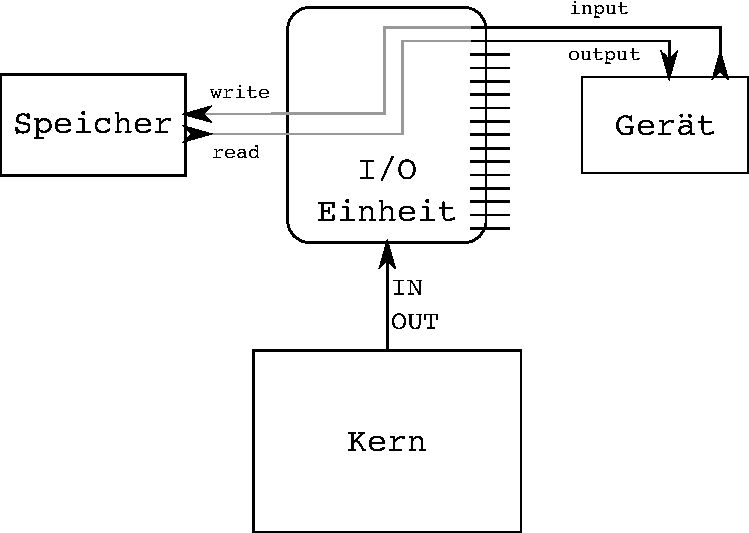
\includegraphics{./img/UMach-IO-Prozess.pdf}
 \caption{I/O wird von der I/O Einheit erledigt}
 \label{fig:UMach-IO-Prozess}
\end{figure}

Alle I/O Operationen finden zwischen dem Speicher und den Peripherie-Geräten
statt. Dabei wird der gesamte Datentransfer von der I/O-Einheit vermittelt und
gesteuert (siehe Abbildung \ref{fig:UMach-IO-Prozess} auf Seite
\pageref{fig:UMach-IO-Prozess}). Die I/O-Einheit besitzt zu diesem Zweck einen
direkten Zugriff auf den Speicher und kann dort unabhängig vom Kern lesen und
schreiben (Direct Memory Access, DMA\index{DMA}). Es ist zu bemerken, dass
der direkte Speicherzugriff von der I/O-Einheit unternommen wird und nicht von
den peripherischen Geräten selbst.

Alle I/O Operationen werden vom Kern unter Programmkontrolle angestoßen (siehe
auch Abschnitt \ref{sec:IO-Instruktionen} auf Seite
\pageref{sec:IO-Instruktionen}). Es werden also keine I/O Operationen
ausgeführt, die nicht explizit durch Maschinenbefehle angefordert werden.
Insbesondere werden keine I/O-Operationen aufgrund von
Unterbrechungsanfoderungen (interrupts) initiiert.

Wenn ein I/O-Befehl ausgeführt wird, delegiert der Kern die Ausführung an die
I/O-Einheit und wartet, bis diese fertig ist. Erst wenn die I/O-Einheit
mit dem Transfer zwischen Speicher und Peripherie fertig ist, fährt der Kern mit
dem Programmablauf fort. Es werden parallel keine Instruktionen aus dem
Speicher geholt oder ausgeführt.


Die I/O-Einheit der UMach Maschine besteht aus einer Reihe von jeweils 8
Eingangs- und Ausgangschnittstellen, auch Ports\index{Port}\index{UMach!Port}
genannt. An diesen Ports können verschiedene physikalische Geräte angeschlossen
werden, welche die entsprechenden Daten generieren bzw. verarbeiten können.
(Siehe Abbildung \ref{fig:umach-aufbau} auf Seite \pageref{fig:umach-aufbau}.)


Die I/O Ports sind in zwei Kategorien unterteilt: 8 Eingabeports und 8
Ausgabeports. Von der Bauart und Struktur her, gibt es innerhalb der jeweiligen
Kategorie keine Unterschiede zwischen Ports. Sie werden lediglich anhand deren
Nummern identifiziert. Die Nummerierung der Ports fängt bei 0 an und wird bis
einschließlich Port 7 fortgeführt. 


Die Eingabe- und Ausgabefunktionen der I/O-Einheit werden durch
I/O-Instruktionen angefordert. Diese Instruktionen werden im Abschnitt
\ref{sec:IO-Instruktionen}, ab der Seite \pageref{sec:IO-Instruktionen}
beschrieben.


\paragraph{Bemerkung}
Zu diesem Entwicklungspunkt sind für die peripherischen Geräte, bzw. für die
entsprechenden Ports keine Kontrolle- oder Statusregister vorgesehen. Es gibt
auch keine entsprechende Befehle für die Kontrolle und Statusabfrage der
peripherischen Geräte. Es wird lediglich in den Speicher eingelesen und aus dem
Speicher ausgegeben. Kontrolle und Statusabfrage sind als Software-Protokoll
gedacht und nicht als Hardware-Vorgang.
